\chapter{绪论}\label{chapter_introduction}
硼化合物自从人类文明开始以来被广为使用,如古代陶器制作中所
上色的釉彩就用到了硼化物。进入现代社会之后,硼化物在各个领域得到了更为广泛的
应用,比如超硬材料、半导体、医用药材等,目前硼化物在材料大家庭中正日益扮演着
更加重要的角色\cite{albert2009boron}。

\section{二维过渡金属硼化物研究进展}

硼元素作为周期表中碳元素的近邻元素有三个价层电子,由于其不能够通过经典的二中心二电子(2c-2e)硼-硼键形成满足八电子规则的构型,硼元素在形成化合物时会展现出极其丰富的成键形式,这个原因导致了硼的化合物有极为丰富的结构多样性。
稳定的硼材料中通常都存在缺电子的成键类型,比如,在许多硼材料中都能够发现三中心二电子键(3c-2e)的存在。其中,二维硼平面的多样性丰富且存在许多新奇的物理化学性质。
近些年,基于硼元素的二维材料设计吸引了广泛的研究关注。大量的二维稳定硼结构被理论预测报导,其中一些还展现出非常优秀的电学、力学性质,如能带中存在狄拉克锥、力学上有高的延展性等。
理论预测硼元素在特定的金属衬底上更易成核并生长为二维材料\cite{liu2013probing,liu2013boron,zhang2015two},依据该结论三个不同的研究组分别成功在不同衬底上合成了二维硼材料\cite{mannix2015synthesis,zhong2017metastable,zhong2017synthesis,li2018experimental,feng2016experimental} 。

过渡金属因为外层具有未满的$d$轨道,其形成化合物时存在许多可变的价态,这个原因导致含有过渡金属的化合物会表现许多丰富的物理化学性质。硼和金属形成化合物,如在硼平面或硼团簇中嵌入金属元素,尤其是过渡金属元素,使得硼元素化合物在结构多样性更加的丰富,同时也可能产生更为丰富的物理化学性质。在这一节我们将介绍二维硼材料的结构多样性,以及在二维硼中嵌入过渡金属元素后,所得到的新颖化合物及其性质的理论计算方面的研究。

\subsection{二维硼材料结构与稳定性}
石墨烯\cite{novoselov2005two, zhang2005experimental, ferrari2006raman,yan2012first, lu2009tuning}的发现,
使得二维材料如硼氮平面\cite{watanabe2004direct},硅烯\cite{liu2014comparison, molle2018silicene, li2018stable},锗烯\cite{liu2015multiple},
磷烯\cite{hu2018strong},过渡金属双硫化合物\cite{cai2014constructing, wang2012electronics, pei2015exciton},砷烯\cite{zhang2015atomically}等,
在近十多年间得到了广泛的研究关注,而且有越来越多的二维材料被实验合成或被理论预测报导。
由于二维材料独特的物理化学性质(如费米能级附近的高导电性,高导热性,高机械强度),二维材料在电器件、能源储存等领域有重要的应用前景。
从2015年第一次在银衬底上合成硼平面至今,二维硼结构的研究在凝聚态物理、化学和纳米材料领域得到快速的发展和广泛关注。由于其独特的物理化学性质,二维硼材料有很大的应用前景和研究价值。

硼烯是由硼原子所构成的单层结构,它能够在高真空环境下生长在银衬底上\cite{zhang2015two}。
被实验合成的四个相为:2-$Pmmn$, $\beta_{12}$, $\chi_3$, 蜂窝相,如图\ref{fig:boron4phase}所示,这四个相均为金属性。性质方面,有研究分别报导了其机械性能、电子结构、晶格热导、超导、原子吸附等\cite{penev2016can, xu2016nucleation, lopez2016electronic, peng2016electronic, carrete2016physically, wang2016strain, xiao2016enhanced, gao2017prediction, liu2016stable, yang2008ab, zabolotskiy2016strain, yuan2015effect, liu2013boron, zhang2016borophene, shu2016unveiling},我们将在该小节后续内容中展开介绍这些性质方面的研究工作。
由于硼平面的能量相比于体相的硼高出了不少,因此硼平面的合成难度很大。其中2-$Pmmn$相的硼平面的能量和$\alpha$-六方晶系的体相硼之间的能量差为\SI{555}{\meV/atom}\cite{lherbier2016electronic}。已经被合成的二维硼的四个结构相均是在实验合成之前就已经被理论预测所报导,这展现了理论预测的巨大作用。扫描隧道显微镜(STM)获取的的图像和结构的建模如图\ref{fig:boron4phase}所示,其中硼烯2-$Pmmn$相显示很大的各向电子异性,同时实验还报导了它特殊的机械性质。该相在衬底上呈褶皱分布,隆起处垂直方向的高度为\SI{0.91}{\angstrom}。$\beta_{12}$和$\chi_3$相可以在银的(111)面衬底上合成,这两相都是平面结构,竖直方向上没有隆起,两相的区别在于水平方向上的硼原子和空位分布是不同的。
2019年研究人员在铝的(111)面衬底上生长得到的石墨烯形状的硼烯结构\cite{li2018experimental},该结构在铝(111)面衬底上比在银(111)面衬底上要稳定的多。原因是,与石墨烯相比,该硼烯中每个硼原子有一个电子的缺失,但银衬底相比铝衬底更不容易出现电荷转移,铝向硼平面转移了更多的电子从而稳定结构。这四个稳定的二维硼烯的合成大大激励了研究人员对硼烯的研究热度,同时也为硼烯在纳米器件和能源领域的应用提供了可能。

\begin{figure}[bt]
  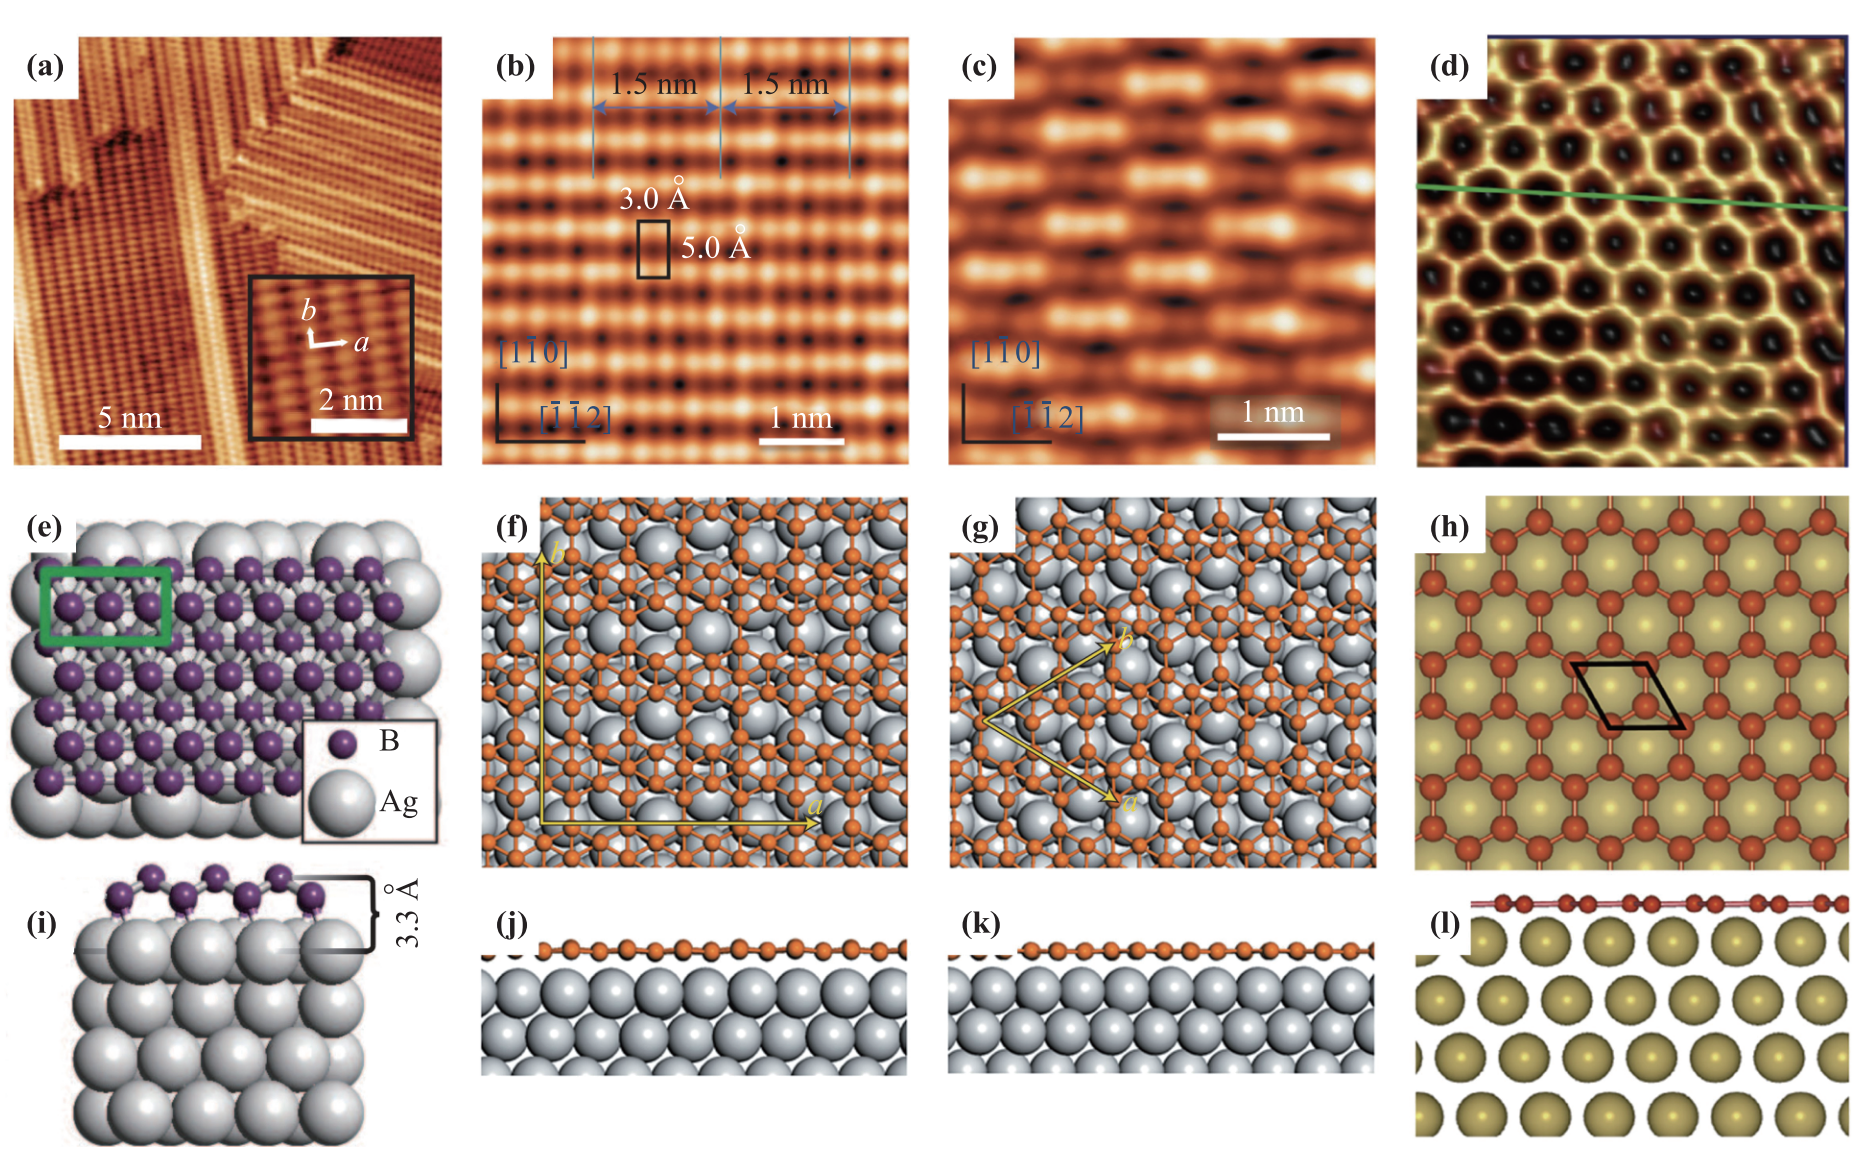
\includegraphics[width=1.0\textwidth]{figs/ch1_boron4phase.png}
  \centering
  \caption{硼在银/铝衬底上生长的2-$Pmmn$, $\beta_{12}$, $\chi_3$, 蜂窝相,(a-d)为STM电镜图,(e-h)为俯视图,(i-l)为侧视图,图片来源并整理自文献\cite{mannix2015synthesis,li2018experimental,feng2016experimental}}
  \label{fig:boron4phase}
\end{figure}

其它的二维硼的同素异形体都是由理论预测所报导的\cite{liu2018intermixing, liu2013probing, penev2012polymorphism, zhang2017elasticity, zhao2016superconductivity, yang2008ab, zhang2016polyphony, tsafack2016thermomechanical, zhang2016substrate, ma2016graphene}。
硼烯的稳定性与硼平面中空位的浓度有重要的联系,我们设平面三角网格中六角空位的比例为$x$,则$x$可能的取值必定在完全的三角网格和石墨烯形的六角格子的空位率之间。
如图\ref{fig:ch1_formation_boronphenes}所示,硼平面的形成能的空位率的变化呈现V型的关系,即从完全的三角格子向六角格子过渡,形成能先随着空位率的增加而降低(变得更稳定),在达到一定数值后又随着空位率的增加而升高(变得不稳定)。在空位率为$x=1/9$时\cite{penev2012polymorphism},可以得到对应的最为稳定的结构,同时在相近的空位率为$x=1/8$和$x=2/15$时,同样有很低的形成能,因此认为这些结构都有可能稳定地存在。
与其他二维材料如石墨烯、硅烯、锗烯、氮化硼以及黑磷所不同的是,硼烯的各种平面结构中在最稳定的结构附近,存在大量形成能相近的构型。

\begin{figure}[bt]
  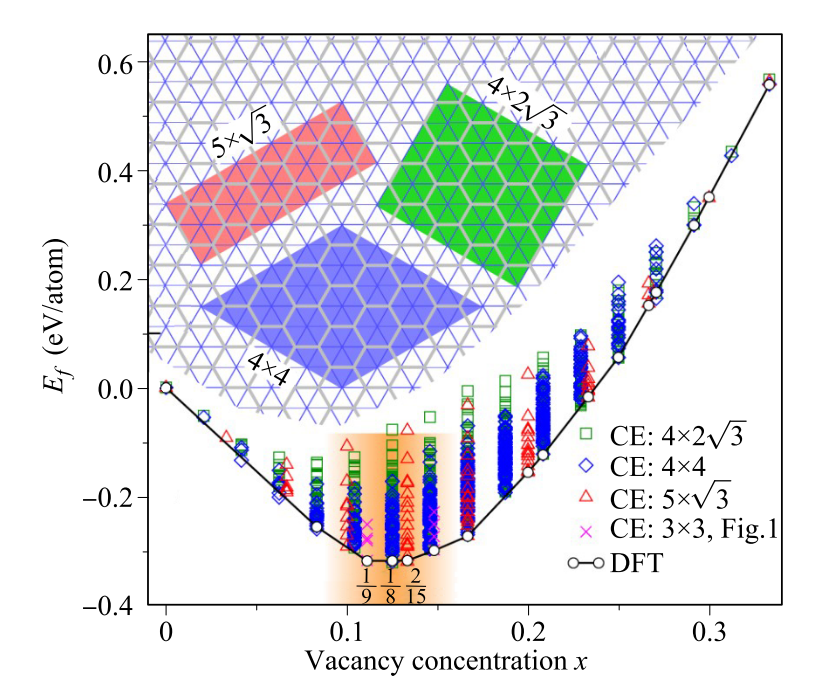
\includegraphics[width=1.0\textwidth]{figs/ch1_formation_boronphenes.png}
  \centering
  \caption{硼平面形成能$E_f$与硼平面空位率$x$的关系,图片来源文献\cite{penev2012polymorphism}}
  \label{fig:ch1_formation_boronphenes}
\end{figure}

除了和空位率相关,如前面所列举的,硼烯的稳定性还受到了衬底的影响。
Yakobson等人提出\cite{zhang2015two},无衬底时的基态结构虽然形成能较低,但生长在衬底时却不一定是最稳定的。
如图\ref{fig:ch1_borophene_energy_spectra}所示,在银的(111)面衬底上,$\beta_{12}$相是最稳定的硼烯,其空位率为$x=1/6$.第二稳定和第三稳定的构型的空位率分别为$x=1/8$和$x=1/12$。
相应的形成能比最稳定的$\beta_{12}$构型要高出\SI{0.4}{\meV}和\SI{2.1}{\meV}。
在铜的(111)表面上能量最低的三种构型的空位率均为$x=1/6$,相比于能量最低的构型,次低和第三稳定的构型的形成能分别高出\SI{15.1}{\meV}的\SI{28.9}{\meV}\cite{zhang2015two}。这个结果表明,在铜的衬底上更有可能形成特定的统一的硼烯构型。

\begin{figure}[bt]
  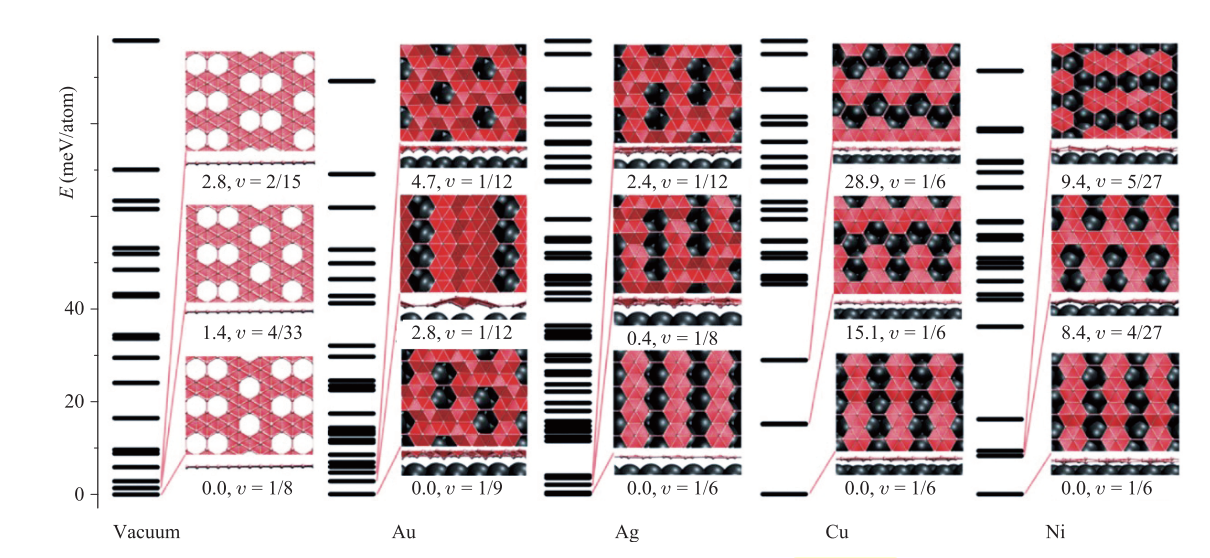
\includegraphics[width=1.0\textwidth]{figs/ch1_borophene_energy_spectra.png}
  \centering
  \caption{理论预测硼烯在金、银、铜、镍衬底上生长的能量谱,图片来源文献\cite{zhang2015two}}
  \label{fig:ch1_borophene_energy_spectra}
\end{figure}

除了空位率和衬底外,官能团修饰是调节硼烯物理和化学性质的另外一个有效手段。比如在其他二维材料如石墨烯、硅烯、锗烯中,
能够使用氢化的方法来增加半导体材料的带隙,或打开金属性材料的带隙将材料从金属变为半导体\cite{balog2010bandgap,bhattacharya2011strain,houssa2011electronic}。
同时官能团修饰后的材料在结构上也会发生明显的改变。石墨烯是完全平面的二维材料,但完全氢化后石墨烯结构呈现隆起状。
与石墨烯类似,硼烯也同样能通过官能团修饰的方法改性,通过氢化能改变硼平面结构的稳定性,比如对2-$Pmmn$相的硼烯进行氢化,声子谱在$\Gamma$点处的虚频消失,结构上更加稳定\cite{xu2016hydrogenated,wang2016high}。
氢化还会改变构型的电子结构\cite{xu2016hydrogenated},在对2-$Pmmn$相的硼烯氢化后,原结构对应电子结构中电子占据的反键部分的电子向氢原子发生转移,使得面内的成键轨道完全占据,反键轨道无占据,从而使结构更加稳定。而且,该氢化后的结构在布里渊区的$X-\Gamma$方向存在狄拉克锥的电子结构,狄拉克点处的电子速度为\SI{3.5e6}{\metre\per\second}\cite{xu2016hydrogenated}。另外,氢化后结构的力学性质也得到了改善,其面内两个方向的杨氏模量分别为\SI{172.24}{\N\per\meter}和\SI{110.59}{\N\per\meter}\cite{wang2016high}。

\subsection{二维硼材料的性质}
热传导性能是纳米器件使用性能和耐用性的重要指标。
有一系列的文献\cite{li2018stretch, mortazavi2018borophene, zhou2017superior, liu2017anisotropic, sun2016first, mortazavi2017anomalous}报导了二维硼材料有关这一性质的研究。
硼烯2-$Pmmn$相为各向异性,其热导也表现出极大的各向异性。室温时,2-$Pmmn$相沿锯齿状(zigzag)方向和沿椅式状(armchair)方向的热导分别为\SI{75.9}{\W\per\meter\per\kelvin}和\SI{147.0}{\W\per\meter\per\kelvin}。这两个方向的声子平均有效自由路程为\SI{16.7}{\nm}和\SI{21.4}{\nm}。
$\alpha$-硼平面具有各向同性,其热导为\SI{14.34}{\W\per\meter\per\kelvin}。硼烯中热导主要是由高频声子的振动模式所贡献的,这不同于在其他二维材料如石墨烯,硅烯,磷烯,这些材料的热传导性质主要是由低频的声子模式所决定的\cite{gu2015first,qin2015anisotropic}。

从实验上合成得到的单层硼平面结构,研究人员对其进行了系统的电子结构性质的研究。实验测试和理论计算的结果显示,得到的单层硼烯平面,原子起伏的2-$Pmmn$相,$\beta_{12}$相以及$\chi_3$相,都是金属\cite{shu2016unveiling},Yakobson等人\cite{penev2016can}通过理论计算预测,这种金属单层硼平面应该具有超导电性质。同时,他们还进一步研究了该类金属二维材料其表面的光学性质\cite{huang2017two}。
Feng等人\cite{feng2017dirac,feng2018discovery}通过角分辨光电子能谱(ARPES)测量技术揭示(如图\ref{fig:ch1_boron_arpes}),在实验上对应的两种单层硼的相的电子结构能带中存在非平庸的狄拉克点,因此认为其有可能是二维拓扑材料。
之后,又有进一步的理论计算工作预言了在其他类型的单层硼平面的能带结构中,不但存在各项异性的狄拉克锥, 而且还存在有节线(node-line)特征的非平庸的色散关系\cite{zhang2017dirac}。
Du等\cite{jiao2016two}的理论工作指出,六角晶格的单层硼平面,如果硼原子表面用氢原子修饰,也会实现各向异性的狄拉克点。

\begin{figure}[bt]
  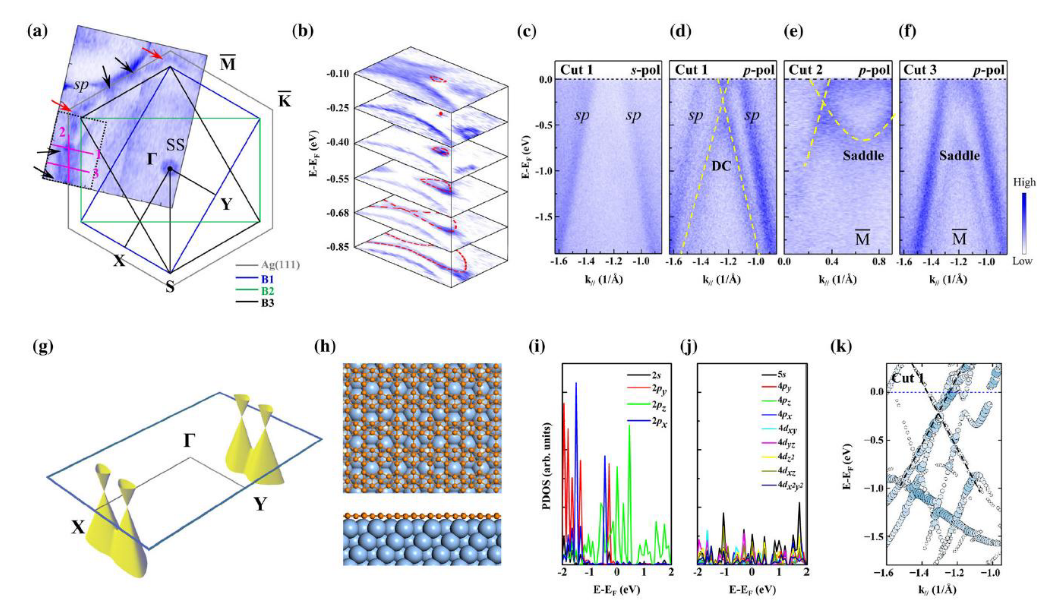
\includegraphics[width=1.0\textwidth]{figs/ch1_boron_arpes.png}
  \centering
  \caption{实验和理论计算的的$\beta_{12}$相在银(111)衬底上的电子能带结构,图片源于文献\cite{feng2017dirac}}
  \label{fig:ch1_boron_arpes}
\end{figure}

需要提及的是,理论预测不但辅助实验合成得到了二维单原子层硼平面,理论还预言了硼存在二维薄膜结构。然而,到目前为止并没有发现硼的层状体相材料的存在,目前已知所有的硼的体相构型都具有高配位的极其复杂的成键方式。如果使用全局构型搜索的方法,当不限制搜索时二维的材料的厚度时,有理论工作表明,多层的硼结构会比孤立单层硼平面更加稳定。
比如Zhou等人\cite{zhou2014semimetallic}通过遗传算法理论预测了稳定的非单层的有狄拉克点的二维硼材料。
Du等人\cite{ma2016graphene}的也发现了一种新型的具有双狄拉克色散的二维硼薄膜。
实验上,2015年南京航空航天大学科研团队在铜表面以硼和\ce{B2O3}为前驱体,通过加\ce{H2}还原的方式得到了二维硼薄膜\cite{tai2015synthesis},该硼薄膜被认为是从体相硼$\gamma_{28}$中切割出的单层结构。
他们理论计算表明,该硼薄膜材料是一种宽直接带隙的半导体材料,其相应的带隙值为\SI{2.07}{\eV},使其有可能被作为具有优秀光吸收性质的材料。
然而,后续又有其他的理论工作\cite{kou2016high}认为这种二维薄膜其实是金属,但如果在其表面通过氢原子进行修饰,可以容易的实现金属和半导体之间的调控。

单层硼平面的结构多样性非常丰富,然而,大多数理论计算和实验发现的单层硼平面都是金属\cite{zhang2017two},Yakobson等人\cite{penev2012polymorphism,penev2016can}在多篇文献中认为,单层硼平面之所以呈现金属性,是因为其体系的费米能级一定会穿过由体系构型中平面结构面外垂直方向的$p_z$ 轨道所构成的能带。
但是体系本身的面内轨道($s$, $p_x$ 和 $p_y$轨道) 在费米能级处是可能存在带隙的。
所以普遍的观点认为,单层硼平面所有构型都不会表现出半导体性质。但我们课题组2017年的工作\cite{xu2017two}报导了理论预测的表现为半导体的几种硼平面构型,这大大的拓展了硼平面的性质。

对于石墨烯结构,可以将孤立的锂原子吸附在石墨烯表面。有理论计算指出\cite{profeta2012phonon},通过控制锂元素的覆盖度变化,可以得到不同的超导转变温度的二维超导体。随后,有另外的研究者\cite{wu2016lithium}将同样的思路拓展到单层硼平面的锂吸附性质上,通过结合集团展开来评估体系能量,他们预测了一系列随覆盖度变化而变化的\ce{Li/B} 超导体,其中所预测的\ce{Li2B7}构型的超导转变温度为\SI{6.2}{\kelvin}。 该研究说明了,通过控制覆盖度以及平面上的孤立原子的吸附位点,可制备出一系列超过液氦温度的传统BCS二维超导体。也正是这个研究引导了本论文关于钛硼单层超导性质的研究思路。

另外,硼平面的化学活性也有不少的相关研究,因为硼单层平面与金属锂具有强的吸附作用,被锂修饰的硼单层平面材料可以被设计用来作为高性能的储氢材料。
有理论\cite{li2015ultrahigh}预测稳定了具有$x=1/8$空位浓度的硼单层平面可能具有较理想的储氢性能。并且,实验上合成得到的硼平面结构也被用来实现锂离子电池的设计。
通过理论计算\cite{jiang2016borophene}发现,2-$Pmmn$相的起伏三角格子的二维硼结构沿其起伏形成的通道方向,其锂离子的扩散非常容易,对应的扩散势垒仅有\SI{2.6}{\meV}。
并且,实验上所合成得到的两种基态构型$\beta_{12}$相和$\chi_3$相本身就有较多的空位的分布,空位连接成链时其可以被看作是理想的离子扩散通道\cite{zhang2016borophene},但不理想的是,由于硼原子的缺电子性,这些空位对应的是较强的金属吸附,导致了锂原子沿这类链状空位路径扩散时的势垒约为\SI{0.6}{\eV}。
如下图\ref{fig:ch1_lina_borophene}所示,分别是$\beta_{12}$相和$\chi_3$相锂离子扩散和钠离子扩散的模拟路径。
相比于其他的二维材料,单层硼烯具有较大的吸附能。
理论计算表明\cite{ling2017nanosheet},在实验上单层$\beta_{12}$平面的六角空位处吸附孤立的金属原子铋,可以作为一个非常有效的单原子催化载体从而可以实现水分解,$\beta_{12}$平面还可作为绿色环境材料用于实现对温室气体\ce{CO2}的高效捕获\cite{tan2017borophene}。

\begin{figure}[bt]
  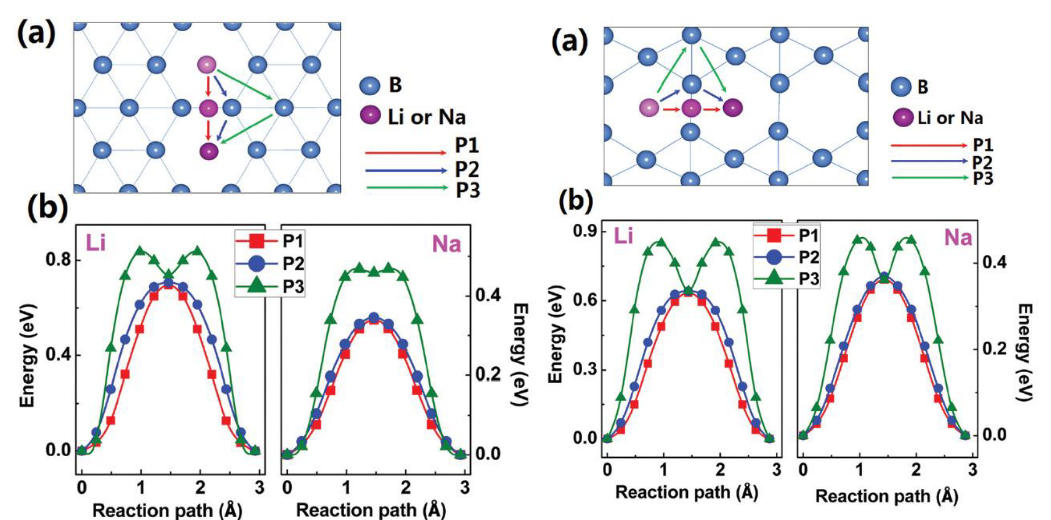
\includegraphics[width=1.0\textwidth]{figs/ch1_lina_borophene.png}
  \centering
  \caption{理论模拟的锂/钠离子在$\beta_{12}$和$\chi_3$表面的扩散路径,图片源于文献\cite{zhang2016borophene}}
  \label{fig:ch1_lina_borophene}
\end{figure}

\subsection{过渡金属硼平面及其理论计算研究进展}
研究原子团簇结构和性质之间的关系,对理解化学键本质以及设计性质可调控的纳米材料有重要的意义。
硼原子由于其缺电子性,较少的硼原子在形成团簇时倾向于形成平面团簇结构\cite{xu2017practical},这一特征和硼的体相结构及体相含硼化合物中的硼复杂网络结构形成鲜明对比。
硼的阴离子团簇最大可达到23个原子\cite{alexandrova2004molecular, alexandrova2004electronic, kiran2005planar, alexandrova2006all, sergeeva2008photoelectron, huang2010concentric, sergeeva2011all, piazza2012photoelectron, sergeeva2012b22, zhai2003hydrocarbon, zhai2003hepta},
在硼原子数量为16的硼阳离子团簇和硼原子数量为20的中性硼原子团簇中,均发现了结构从二维到三维的转变\cite{kiran2005planar, tai2012structure, oger2007boron}。
所有实验发现的硼平面团簇\cite{romanescu2013transition},都是由一圈通过二中心二电子(2c-2e)硼硼键所形成的硼环围绕一个中心原子,硼和中心原子通过$\sigma$键连接,整个平面团簇在水平方面形成一个大$\pi$键来稳定团簇。
我们可以注意到,在阴离子硼团簇中,中心原子通常和多个硼原子形成多中心键,一个典型的例子是\ce{B19^-}(\ce{B}@\ce{B5}@\ce{B13})\cite{huang2010concentric},其中就包含两种不同的离域$\pi$键。
这种离域表示了中心硼原子与中间层的\ce{B5}环,\ce{B5}环与最外层\ce{B13}环之间的相互作用。有趣的是,内层的\ce{B}@\ce{B5}结构可以在\ce{B13}环中自由旋转,这使其成为了分子器件的一个潜在候选。

当八个或九个硼原子成环时,可以在环的中央放入金属离子而形成稳定的团簇结构,这两种轮状团簇是有高对称性的轮状分子,其中硼元素组成的环符合$(4N+2)$休克尔规则,使得结构能够稳定存在\cite{zhai2003hepta,alexandrova2004molecular}。
已经被实验报导的有\ce{AlB7^-}($C_{7v}$)和\ce{AlB^-}($C_{8v}$)\cite{galeev2011valence},结构中的铝元素分别和\ce{B7}与\ce{B8}环通过离子相互作用结合,
金属-硼之间的成键并不离域。2013年Romanescu等人通过激光蒸发喷射超快团簇束的方法得到了一系列以过渡金属为中心与硼环形成的轮状分子结构,\ce{Co}@\ce{B8^-}, \ce{Ru}@\ce{B9^-}, \ce{Rh}@\ce{B9^-},\ce{Ir}@\ce{B9^-}, \ce{Nb}@\ce{B9^-}以及 \ce{Ta}@\ce{B9^-} \cite{romanescu2011aromatic,galeev2011valence,li2012transition},
这些实验发现的结构(如图\ref{fig:ch1_boron_wheel01}和图\ref{fig:ch1_boron_wheel02}所示)也同样被理论证实是该化学配比下能量最低的平面团簇结构。

\begin{figure}[bt]
  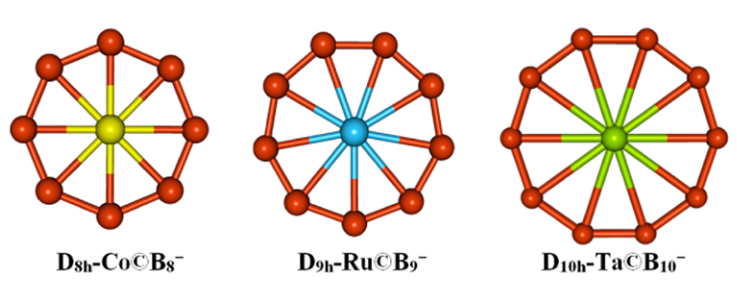
\includegraphics[width=0.86\textwidth]{figs/ch1_boron_wheel01.png}
  \centering
  \caption{轮状结构的\ce{Co}@\ce{B8^-},\ce{Ru}@\ce{B9^-}和\ce{Ta}@\ce{B10^-},图片源于文献\cite{romanescu2013transition}}
  \label{fig:ch1_boron_wheel01}
\end{figure}

\begin{figure}
  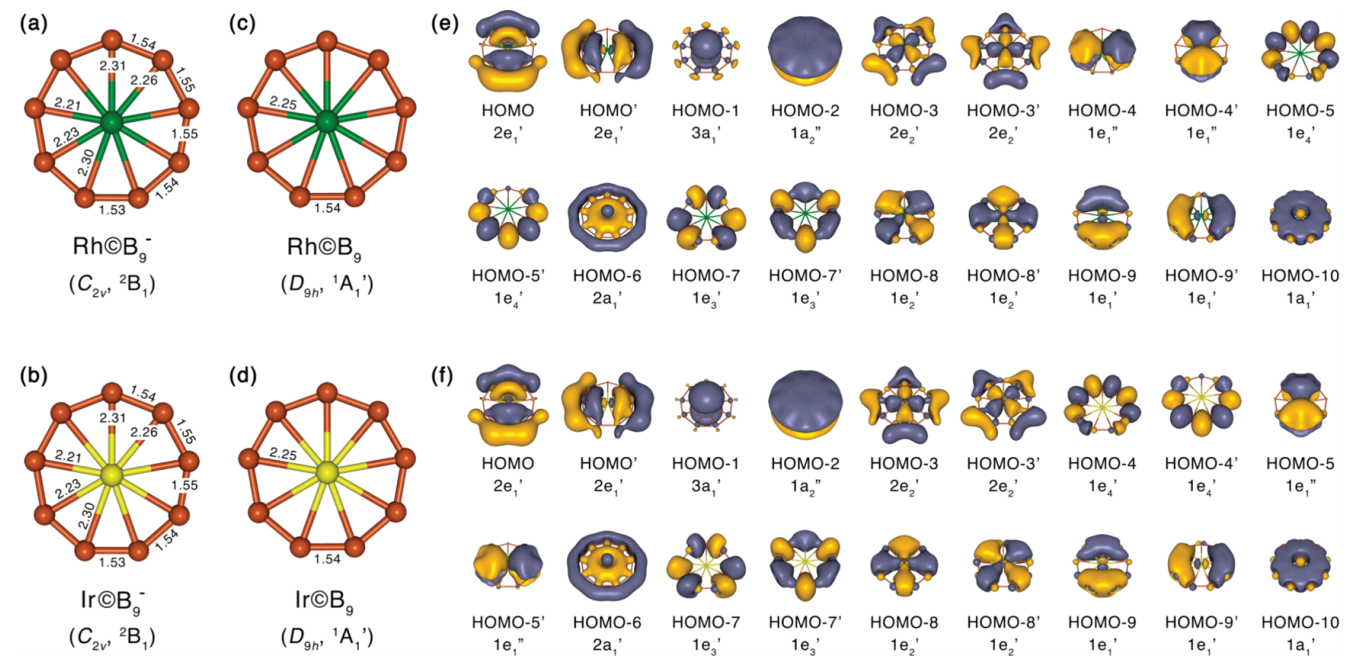
\includegraphics[width=1.0\textwidth]{figs/ch1_boron_wheel02.png}
  \centering
  \caption{优化后的金属硼团簇轮状结构(a)\ce{Rh}@\ce{B9^-},(b)\ce{Ir}@\ce{B9^-},(c)\ce{Rh}@\ce{B9}和(d)\ce{Ir}@\ce{B9}以及理论计算的价层电子分子轨道,图片源于文献\cite{li2012transition}}
  \label{fig:ch1_boron_wheel02}
\end{figure}

\begin{figure}[bt]
  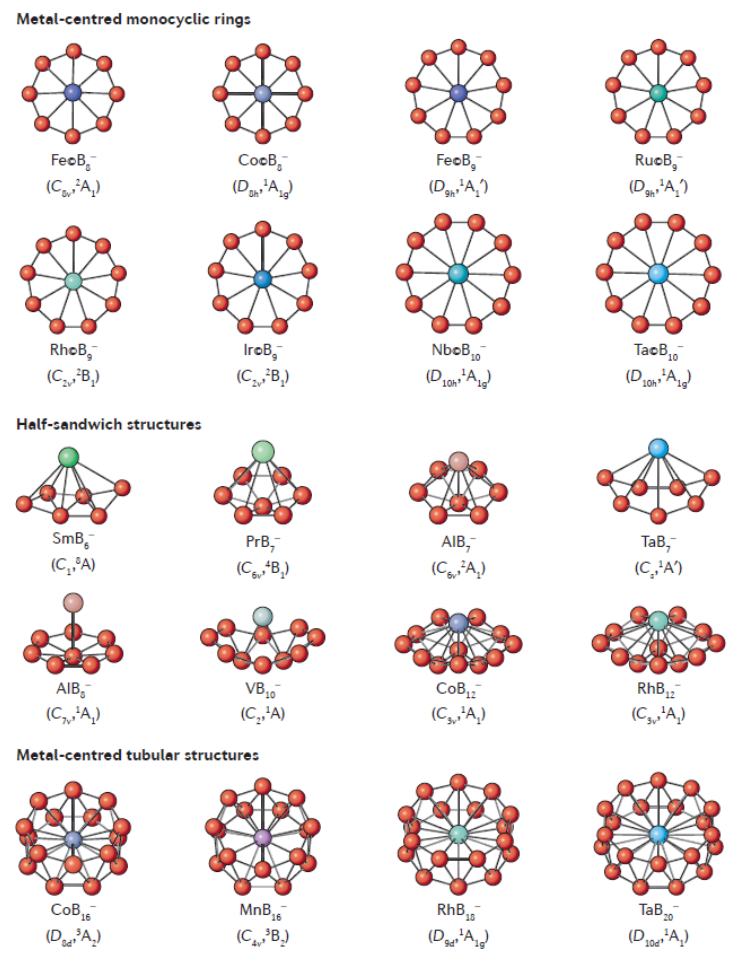
\includegraphics[width=0.96\textwidth]{figs/ch1_boron_metal_cluster.png}
  \centering
  \caption{金属原子与硼团簇结合后形成的稳定纳米结构。本图源于文献\cite{li2017planar}}
  \label{fig:ch1_boron_metal_cluster}
\end{figure}

结合过渡金属与硼形成的轮状结构的稳定性和硼平面的多样性,我们可以将过渡金属硼平面看作是由过渡金属嵌入硼平面中所形成的稳定构型。理论预测报导了许多这样的材料并报导了它们相关的物理化学性质。

Qu等人\cite{qu2017two}使用粒子群算法对钛硼比例为$1:4$的结构进行了搜索,找到了全平的二维单层钛硼结构,如图\ref{fig:ch1_tib4}所示,其中钛原子被八个硼原子环绕形成八配位的钛硼轮状结构,八个硼原子到钛原子的距离均相等。他们计算了该结构的动力学性质,认为其十分稳定因而可能够被实验所合成。同时他们认为该结构的稳定性源于钛和硼形成的八配位的稳定轮状团簇,因为钛向硼提供了电子弥补了硼的缺电性使硼原子之间形成了$sp^2$杂化轨道构成的稳定网络。受该结构启发,他们还对该钛硼结构进行了其他金属原子的替换,将钛替换为钒,镉,锰,钨元素形成平面或准平面结构并讨论了这些结构的稳定性。

\begin{figure}[bt]
  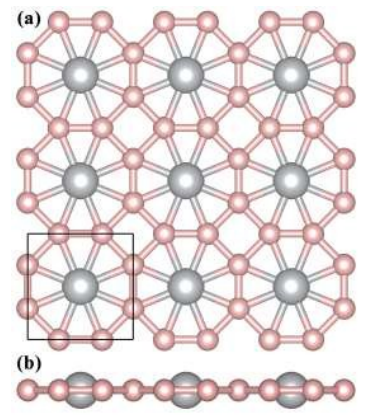
\includegraphics[width=0.42\textwidth]{figs/ch1_tib4.png}
  \centering
  \caption{\ce{TiB4}单层平面的俯视图(a)和侧视图(b),图片源于文献\cite{qu2017two}}
  \label{fig:ch1_tib4}
\end{figure}

Bo等人\cite{bo2019tetragonal}通过第一性原理结合粒子群算法,发现并研究了两种\ce{Mo2B2}单层的稳定性,电子结构,晶格动力学性质以及其在电池材料中作为阴极材料时的性质。声子谱和电子结构的信息展示了正方和三方晶系\ce{Mo2B2}结构(如图\ref{fig:ch1_mo2b2})的高电导性质以及高的稳定性。这两个结构对锂原子和钠原子的吸附能在电池的工作范围内都非常大,确保了其工作效率。其中正方晶系\ce{Mo2B2}的锂离子和钠离子容量均为约\SI{251}{\mA\hour\per\g}, 三方晶系\ce{Mo2B2}的锂离子和钠离子容量分别为约\SI{251}{\mA\hour\per\g}和\SI{188}{\mA\hour\per\g}。
三方晶系的\ce{Mo2B2}对锂离子和钠离子的扩散势垒分别为\SI{0.023}{\eV}和\SI{0.013}{\eV},四方晶系\ce{Mo2B2}对锂钠离子的扩散势垒分别为\SI{0.029}{\eV}和\SI{0.010}{\eV},较低的扩散势垒说明他们有很好的充放电效率。
相同研究组的研究人员还在另一工作中对六方晶系\ce{Ti2B2}\cite{bo2018hexagonal}进行了锂离子和钠离子电池性质的研究,该材料的锂钠离子的容量分别为\SI{456}{\mA\hour\per\g}和\SI{1027}{\mA\hour\per\g}。
值得一提的是该材料对锂离子和钠离子的扩散势垒非常低分别仅为\SI{0.017}{\eV}和\SI{0.008}{\eV},因此推断其具有非常优良的充放电性质。

\begin{figure}[bt]
  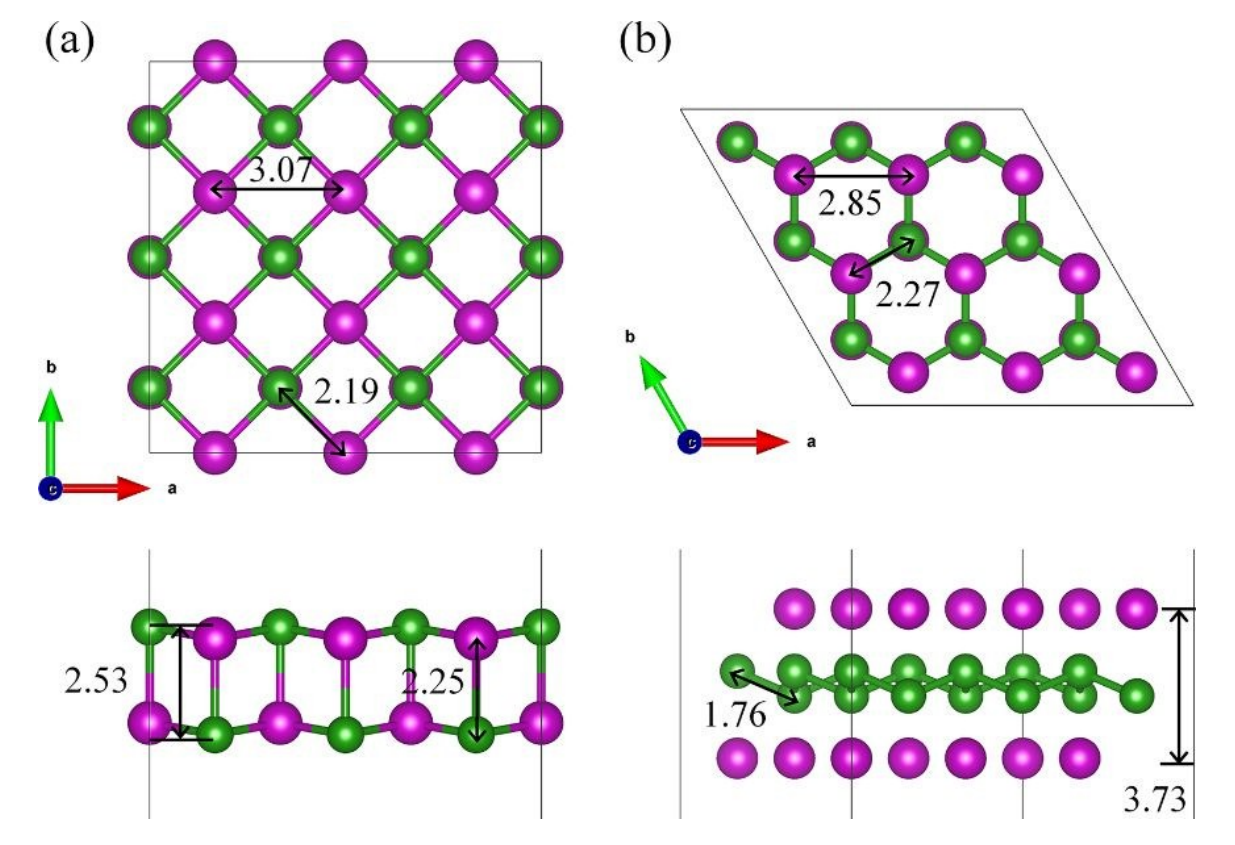
\includegraphics[width=0.86\textwidth]{figs/ch1_mo2b2.png}
  \centering
  \caption{正方和三方晶系Mo2B2结构的俯视图和侧视图,图片源于文献\cite{bo2019tetragonal}}
  \label{fig:ch1_mo2b2}
\end{figure}

Tang等人\cite{tang2019cob}使用粒子群算法预测了钴原子和硼原子形成的单层平面化合物\ce{CoB6}(结构如图\ref{fig:ch1_cob6}所示),并研究了该材料的磁学和电学性质。动力学计算显示该材料有很好的稳定性,同时他们认为该平面\ce{CoB6}是稳定的二维铁磁材料,而且其磁矩和磁稳定性能够通过对材料施加应力来提高。他们还探讨了对该材料可能的合成方法,认为可以通过在已经被实验所报导的$\delta_4$相硼单层平面上,通过吸附钴原子或直接通过化学生长得到该结构。

\begin{figure}[bt]
  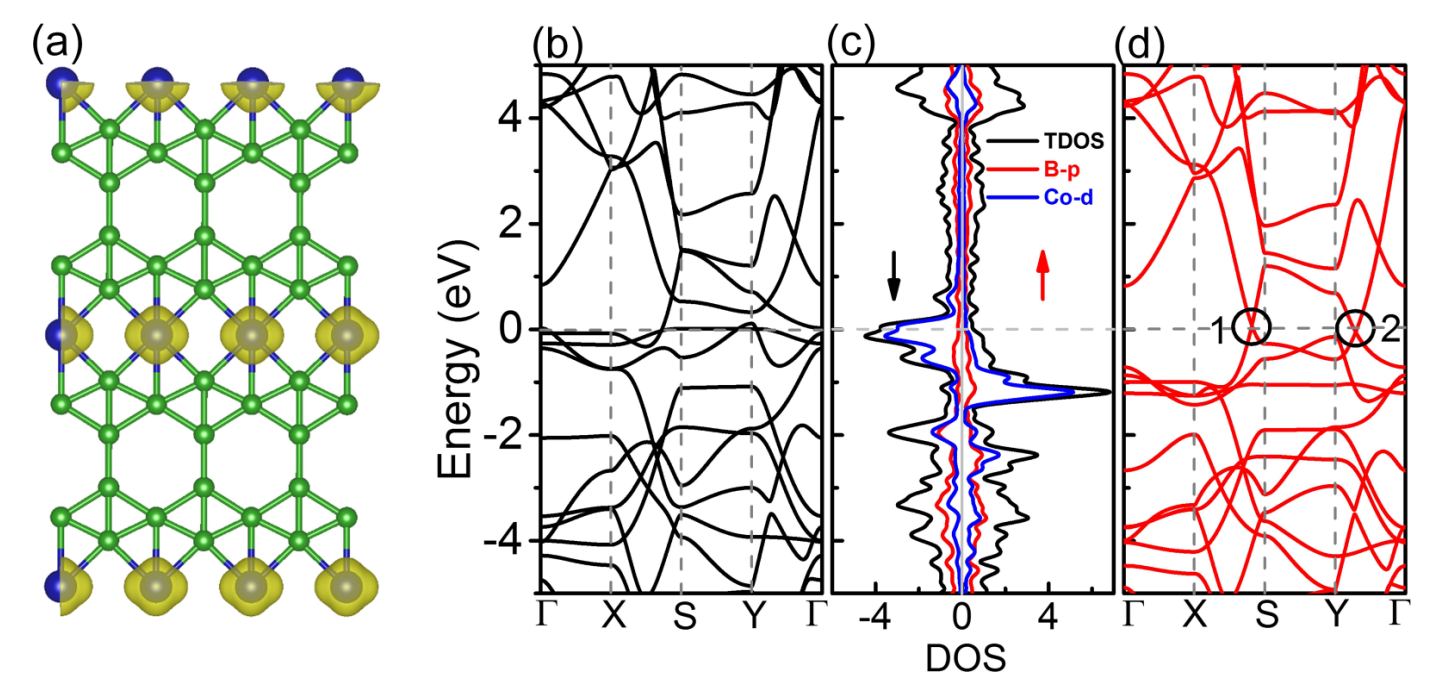
\includegraphics[width=1.0\textwidth]{figs/ch1_cob6.png}
  \centering
  \caption{(a)单层\ce{CoB6}自旋未配对电荷密度分布(b)自旋向下部分的能带(c)态密度(d)自旋向上部分的能带,图片来源文献\cite{tang2019cob}}
  \label{fig:ch1_cob6}
\end{figure}

Wang等人\cite{wang2017semimetallic}通过使用第一性原理计算结合全局搜索算法,发现了一系列\ce{TiB_x}($2\leq x\leq 16$)结构,由钛和硼原子在二维平面排列组成。这些结构因为被钛原子到硼原子的电子转移而更好的稳定。因此,拥有比目前提出的二维硼平面的更好的稳定性。特别是,他们发现了\ce{TiB12}具有足够低的能量,使其可在\ce{TiB2}和二维$\alpha$-硼平面构成的混合物中能够稳定存在。同时,\ce{TiB12}具有带隙为\SI{0.02}{\eV}的准狄拉克点。有趣的是,他们还计算出这种二维\ce{TiB12}材料的功函数和电导率可以通过施加轴向应变进行调节。该二维\ce{TiB12}的合成和新的电子特性使其成为一种有前途的纳米电子应用的新型二维材料。这篇文献中所报导的单层的钛硼平面恰好为本论文的工作提供了充足的参考,本论文的工作在文献所报导的单层钛硼结构的基础上,还得到了一些能量更低的单层钛硼构型并研究了它们的超导性质。


\section{硼化物的超导性质研究进展}

原子质量小的元素所构成的金属材料会展现新颖的电子结构性质,硼作为原子质量较轻的一个元素,单质硼或硼化合物往往会有相对较高的超导温度。
2001年Eremets等人\cite{eremets2001superconductivity}通过金刚石对顶针在超高压160GP下将硼从非金属相转变为金属相,并表现出超导性质,当压力从\SI{175}{\GPa}升高到\SI{250}{\GPa}时,其超导温度从\SI{6}{\kelvin}提升到了\SI{11.2}{\kelvin},即每\si{\GPa}压力增加可提高临界温度\SI{0.05}{\kelvin},理论计算表明该高压材料的超导为BCS机制的超导,对临界温度的理论计算结果与实验测量结果相符合。
同年,Nagamatsu等人\cite{nagamatsu2001superconductivity}报导了具有最高临界温度的非铜氧型的超导体\ce{MgB2}\cite{buzea2001review},其常压下超导温度为39K。
与\ce{MgB2}由相同结构的化合物\ce{AlB2}同样表现出超导性能,但常压下的超导温度为较小,有趣的是能够通过多种手段调节使其超导温度提升。
同类型结构,不同金属元素的\ce{XB2}型化物也同样存在超导性,如\ce{ZrB2},\ce{HfB2}\cite{barbero2017doping},\ce{NbB_{2+x}}\cite{mudgel2008superconductivity}以及\ce{TaB_{2+x}}\cite{singh2001superconductivity}。
这种材料在结构上表现为硼原子以六角格子网络连接,金属原子以插层形式位于硼网络层之间,如图\ref{fig:ch1_mgb2}。这种层状嵌套的结构特征启发研究者们,可能会存在二维的硼或硼化物和超导材料。

\begin{figure}[bt]
  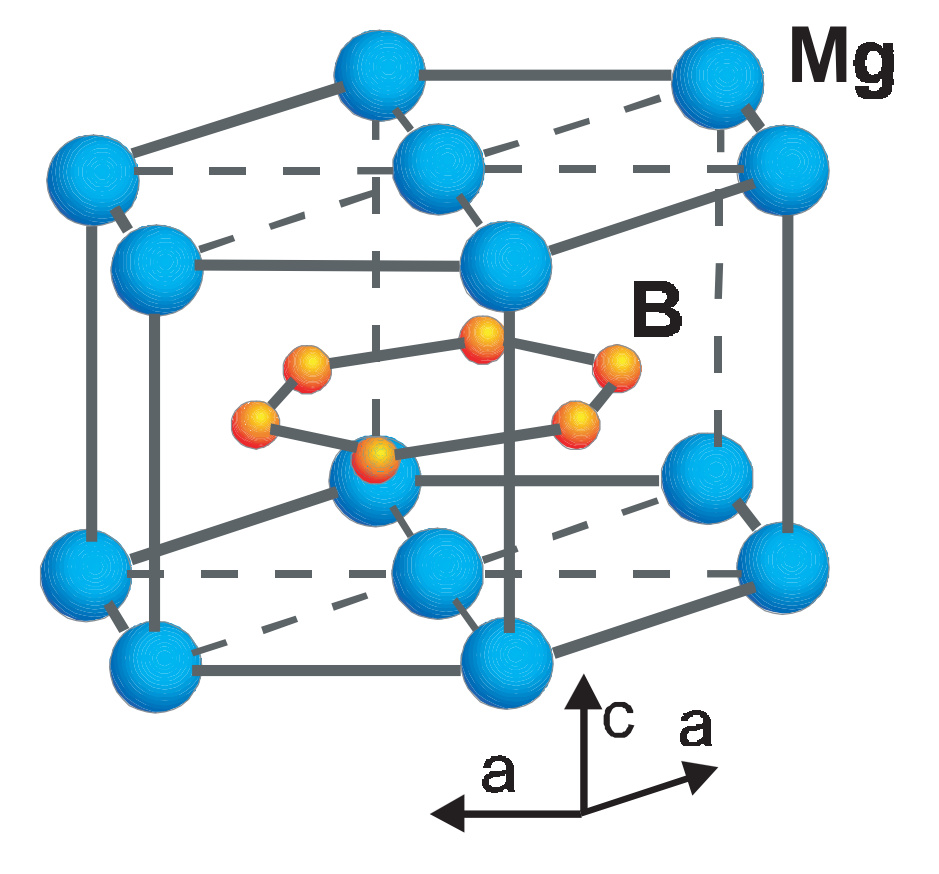
\includegraphics[width=0.60\textwidth]{figs/ch1_mgb2.png}
  \centering
  \caption{\ce{MgB2}(其他元素的超导相由类似结构)的结构图,其中\ce{B}元素形成石墨烯类似的六角格子网络,\ce{Mg}原子嵌入在硼元素组成的六角格子网格堆叠的层之间。}
  \label{fig:ch1_mgb2}
\end{figure}

二维材料的超导性质在纳米超导量子器件\cite{pribiag2015edge}和纳米超导晶体管\cite{el2013superconductivity}中都有重要的潜在应用价值。通过在石墨烯上沉积金属原子的方式,能够使其出现超导性。
2007年首次报导了通过等离子方式在石墨烯上覆盖金属而诱发超导\cite{uchoa2007superconducting},后续的理论计算表明其超导温度为\ce{LiC6}单层8.1K\cite{gholami2018superconducting},和\ce{CaC6}单层1.4K\cite{yang2014superconducting},通过增加石墨烯层数,超导临界温度会发生改变。
与石墨烯类似,硼二维材料也能表现出超导性质。
2017年,Gao等人\cite{gao2017prediction}对实验上能够在银(111)面上生长的$\beta_{12}$和$\chi_3$两种硼平面进行了超导性质的计算,预测其临界超导温度分别为\SI{18.7}{\kelvin}和\SI{24.7}{\kelvin}。
根据2012年Profeta等人\cite{profeta2012phonon}报导的在石墨烯上吸附锂元素能够得到有超导性质的层状结构,2016年Wu等人\cite{wu2016lithium}对锂在硼平面上沉积的结构进行了超导性质的计算,发现了一系列可能稳定存在的锂硼层状超导结构。2019年Yan等人\cite{yan2019prediction}预测了两种稳定的\ce{Mo2B2}结构并计算了它们的超导临界温度为\SI{3.9}{\kelvin}和\SI{0.2}{\kelvin},并发现其电声耦合主要是由于钼原子的低频振动所导致的。

\section{结构搜索与高通量方法在硼材料研究中的应用}

原子在空间中能够以各种各样的形式堆积,从而形成各种类型的凝聚态物质,物质结构,是深入理解物质物理化学性质的非常重要的信息之一。《自然》杂志主编John Maddox曾在《自然》上发表评论称,“依据且仅依据物质的化学组分来确定物质的结构,是物理学的一个重要挑战”。通过计算材料学,从理论上预测和设计具有新颖或优良性质的材料具有极其重要的意义。原因是,理论计算的成本相比于实验较低,且不乏重要的前瞻性,对实验研究中以试错为主要探索方式的方法过程具有很强的指导意义。另外,理论计算的探索和研究,能够帮助研究人员从本质来理解材料结构的其物质性质之间的内在联系,并提供通过结构改变物质性质的关键信息,指导新材料的设计和发现。这样的研究方法对各种物质性质的研究都有着重要的价值。

在过去,科学家只能对已有的材料进行研究,通过实验表征其各种物质性质。因此,对物质性质的改性也往往只能限制在已有的物质结构的基础上,这大大限制了对材料性质的探索。近年来,科学家发展了一些新的结构搜索程序比如基于粒子群优化机制的CALYPSO程序\cite{wang2012calypso}、基于遗传算法的USPEX程序\cite{glass2006uspex}。
仅需要材料元素种类和配比,不需要任何结构信息,就可以产生大量可能的结构, 然后对这些结构进行优化和能量比较, 得出能量较低的结构,可再进一步研究这些结构的各种性质。结构搜索程序的日趋成熟加上服务器计算能力的提高, 极大地推进了探索新型材料的进程。即使对于实验上已经存在的材料,研究者采用结构搜索程序也能对其可能在其他极端条件下存在的未知构型进行进一步的探索和尝试。

硼原子能够组成许多原子数不同尺寸各异的硼团簇,且这些硼团簇具有新奇的电子结构特征。
通过CALYPSO,Wang等人\cite{lv2014b38}2014年报导了38个硼原子组成的硼团簇,该团簇有很好的稳定性,
较大的能带和高的芳香性。如果再引入其他原子,那么硼还能够形成更加丰富的多配位团簇构型\cite{lv2015stabilization},
如图\ref{fig:ch1_boron_cluster01}和图\ref{fig:ch1_boron_cluster02}所示,通过结构搜索算法研究人员找到了一系列金属-硼团簇。
\ce{Li2B24}\cite{dong2019li}为管状结构,具有多重芳香性,能够用于生长硼纳米管。碱土金属镁能够和硼形成具有高稳定性的鼓状结构\ce{MgB18}团簇\cite{tian2019exhaustive}。铍元素能够和硼形成形似的团簇如具有二次旋转轴的\ce{BeB16^-}团簇\cite{kang2019probing}。与硼同处于第13族的铝与硼有相同的价电子结构,铝元素对硼团簇结构的影响较小,但能够增加其稳定性,铝硼能够形成环状平面结构\ce{AlB18^-}\cite{jin2019structural},有很大的带隙和较高的芳香性。
一通过结构搜索方法Tian等人\cite{tian2019cluster}还找到了一大类过渡金属-硼团簇,这给周期性体系过渡金属硼的构建提供了丰富的构型资源。

在二维硼平面的结构搜索中,Wu等人\cite{wu2012two},使用第一性原理粒子群算法,预测了两种稳定的单层硼平面$\alpha_1$平面和$\beta_1$平面,他们的能量均比原先报导的由Tang和Yang等人\cite{tang2007novel,yang2008ab}分别报导的$\alpha$硼平面以及由Yakobson等人\cite{penev2012polymorphism}报导发现的$\beta$硼平面的结合能更低。
利用全局结构搜索软件,Qu等人\cite{qu2017two}预测发现稳定的\ce{TiB4}结构。
Zhang等人\cite{zhang2017dirac}报导发现了能带结构中具有狄拉克锥的\ce{FeB6}结构。

\begin{figure}[bt]
  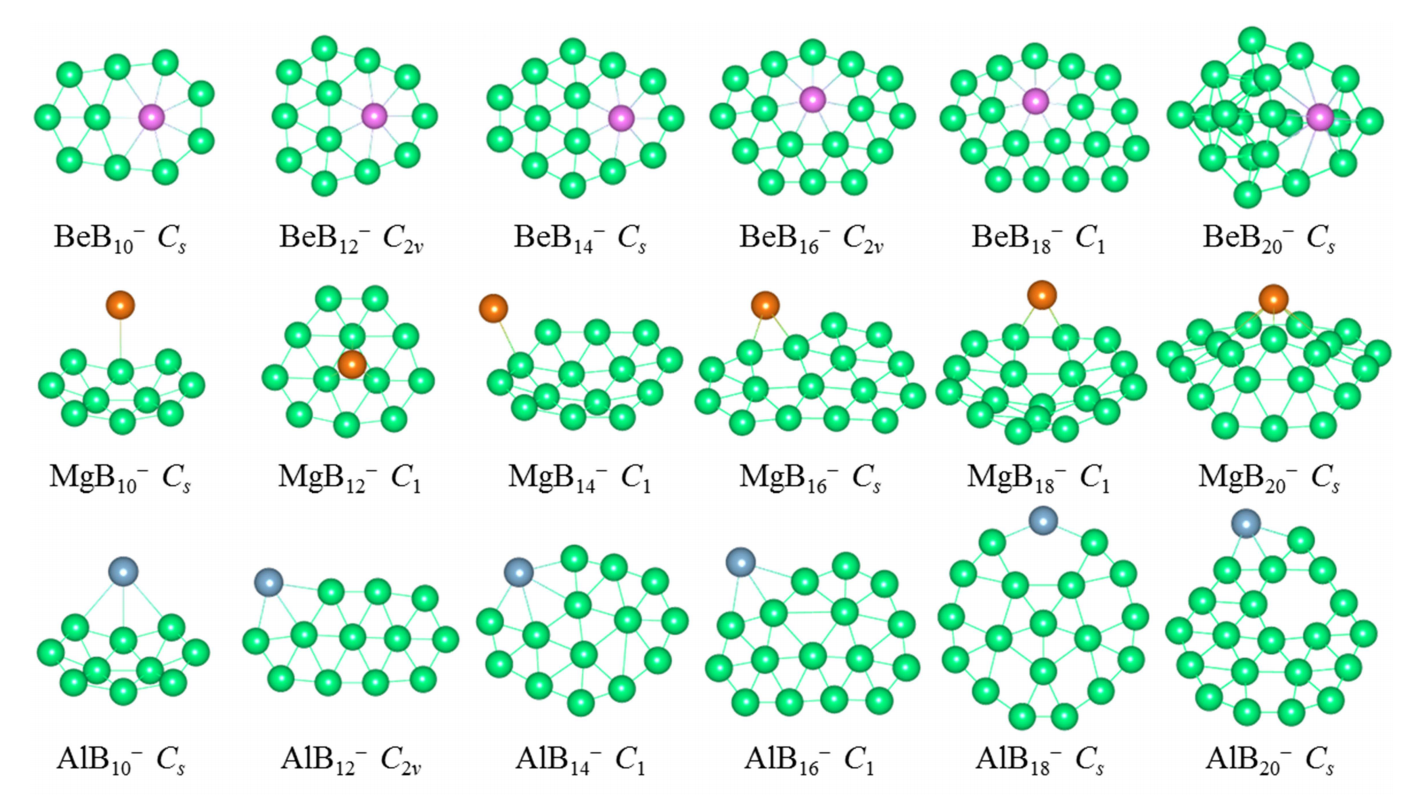
\includegraphics[width=0.96\textwidth]{figs/ch1_boron_cluster01.png}
  \centering
  \caption{金属原子Be,Mg,Al与硼团簇结合后形成的稳定纳米结构。本图源于文献\cite{tian2019cluster}}
  \label{fig:ch1_boron_cluster01}
\end{figure}

\begin{figure}[bt]
  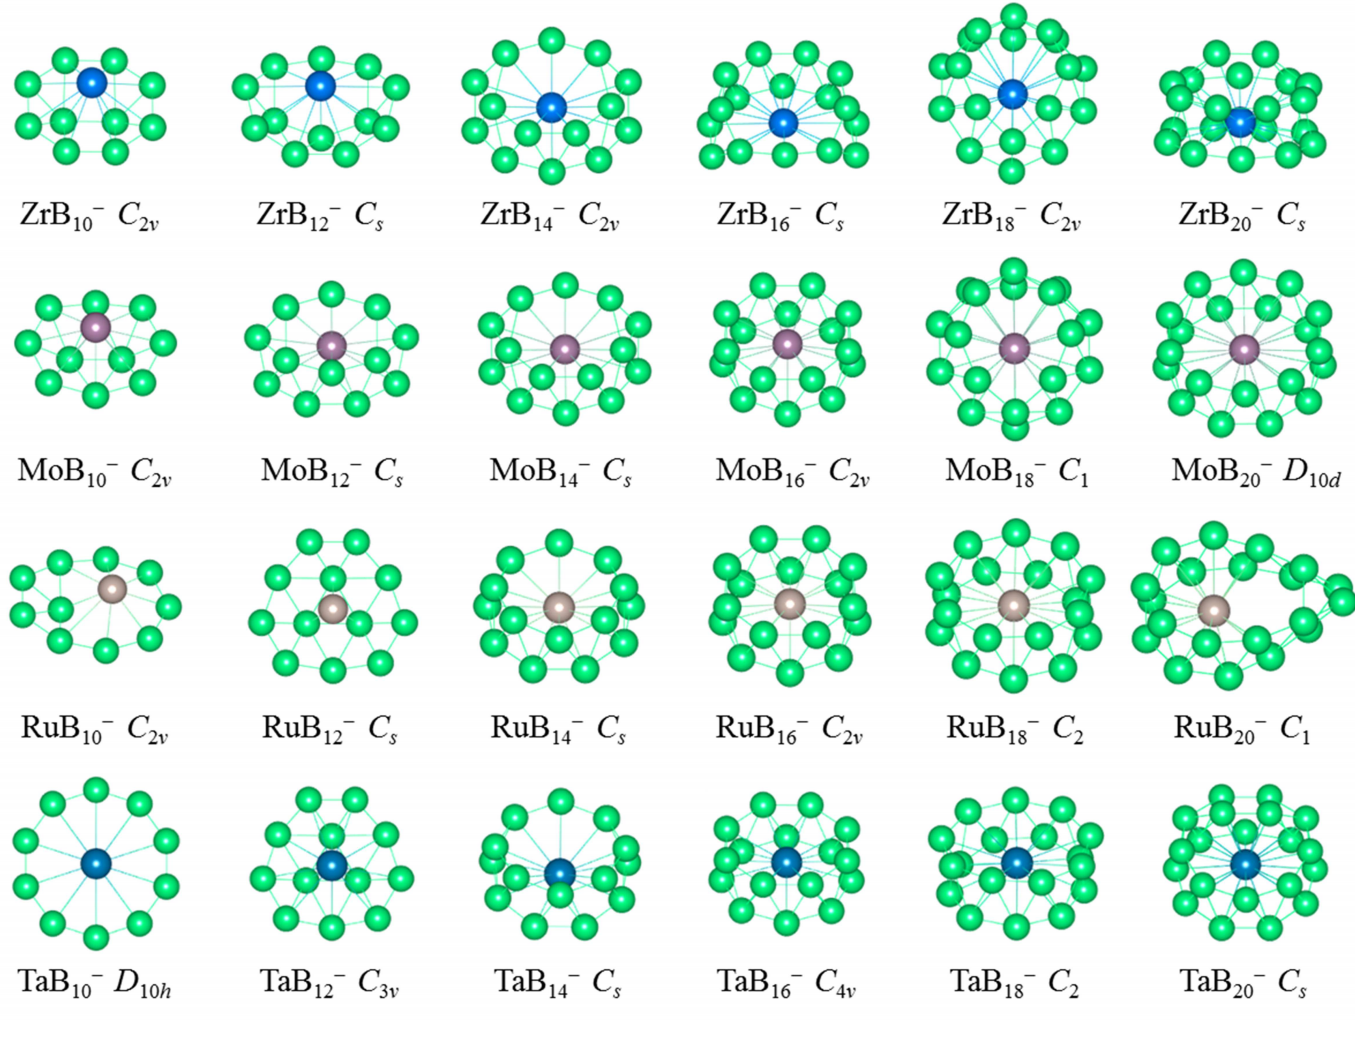
\includegraphics[width=0.96\textwidth]{figs/ch1_boron_cluster02.png}
  \centering
  \caption{金属原子Zr, Mo, Ru, Ta与硼团簇结合后形成的稳定纳米结构。本图源于文献\cite{tian2019cluster}}
  \label{fig:ch1_boron_cluster02}
\end{figure}

高通量计算材料学的方法,是与结构搜索对应的一种结合理论计算和数据分析技术来指导材料制备和研究的方法。
实验科学家通过规律和经验将某种材料合成并生长到能够完整测量其性质的规模往往是一个并不简单,及其耗费时间的过程。
因此材料从发现到实际的工业应用是非常缓慢的。这个过程中的许多步骤往往有极大的可重复性,并且不同材料间很可能因为细微的变量变化而出现性质上的巨大差别。
实验科学家有必要全面的考察各个变量所可能导致的结果差异。而这个过程中,就存在变量以外的如人工的重复。
信息化工业化的今天,将人的精力耗费在不断机械重复特定流程的工作中并不是一个理想的科学模式。
那么,高通量计算材料学就是这样一种方法,将重复的工作交由机械和计算机来完成,以解放科学家的时间和双手,使得科学家能够着眼于问题本身的探索。
今天,高通量实验科学尤其是高通量计算材料学已经发展出一套成熟和完整的方法\cite{curtarolo2003predicting, ceder1998identification, johannesson2002combined, curtarolo2005accuracy, xiang1995combinatorial, koinuma2004combinatorial, takeuchi2003identification}。

高通量计算材料学是使用高通量的方法结合计算材料学进行材料的设计。它是计算材料学与基于数据库构建,数据挖掘的计算机技术的结合。
通过对已有和理论预测的材料进行热力学、电子结构等性质的计算,之后将所得信息储存进入数据库,通过数据挖掘技术来筛选预测可能具备某种特别优秀性质的材料。
这个流程准确地符合了广义上的经验主义的科学方法论,即通过归纳来描述某类共有的科学现象并总结为规律,并且该规律还需要拥有演绎推广和预测未知的能力。我们希望将这个方法发展并应用到具有极大结构多样性的含硼化合物的结构与性质的研究中。

可以看到,硼元素因其独特的缺电子特性,在结构多样性上非常丰富,但同样可以看到,由硼所形成的结构都是由硼元素以密堆的方式形成网络,但由于其缺电子性,网络中需要空位或者其他元素原子作为电子给体来平衡电荷分布。根据以上特征,可以有选择的给出可能稳定的初始结构,使得所需要计算的结构数量大大降低而不再依赖于全局搜索算法。利用这样的方法,我们课题组对硼平面团簇结构进行了高通量结构搜索,对数千个候选结构进行能量的考察,不但能够全数找到已经被实验发现的平面团簇,还预测了稳定的\ce{B76}团簇\cite{xu2017practical}。通过对硼平面使用类似的方法,找到了具有半导体性质的硼平面结构\cite{xu2017two},这是首次发现报导的具有半导体性质的硼平面构型,这些构型的发现丰富了硼平面的性质,增加了硼平面应用上的潜质。在此基础上,我们在本论文的相关工作中将研究对象进一步扩充到了过渡金属和硼形成的二维材料中。通过结合新的高通量方法和工具,我们发现了一系列新的过渡金属-硼二维化合物,并研究了它们的性质。

\section{论文的研究意义和主要内容}
二维硼材料结构和性质上的多样性非常丰富,实验上研究人员已经能够生长出一定尺寸的单层硼材料,理论预测二维硼材料以及硼与其他元素所形成的二维化合物会表现出许许多多丰富的物理化学性质,尤其是当硼和过渡金属原子形成的二维化合物时,理论计算预测了很多新奇的性质,使二维硼化合物不但有应用上的潜力,同时也是很好的新物理现象的研究对象。
但硼在结构上丰富的多样性,一方面是其丰富的性质多样性的来源,但另一方面这也使得其合成和稳定结构的确定变得困难。如何发现和理论预测满足特定结构特定性质的二维硼材料,是本文研究的出发点。如果能从理论上预测具有优秀物理化学性质的二维硼材料,并对预测的材料的结构稳定性、结构特征、材料性质进行深入的研究,则能够指导和加快实验上对此类材料的发现和应用,从而大大减少材料科学中实验的人工成本和材料成本。

针对二维硼材料结构上的共性,我们使用加入结构相关的先验知识进行有偏向性的筛选和搜索(biased-screening)。
结果显示对我们关注的硼化物材料,这种方法的效果会优于使用全局搜索算法的无偏向性的结构搜索(unbiased-screening)。
通过加入硼二维材料中硼原子之间倾向于保持包含空位的硼平面三角网格的结构,我们使用结构查重软件优先构建了尽可能均匀分布于势能面空间中目标结构能量局域极小值点附近的初始构型。
再对所有生成的结构进行第一性原理计算以获得准确的能量和性质。
通过使用这个方法,我们研究了钛硼单层的稳定构型,不但发现了各个不同配比下已经报导过的几个钛硼单层材料,还发现了能量更低且具有优秀超导性质的\ce{TiB7}单层构型。
需要强调的是,通过加入先验的结构信息,我们所生成和计算的结构总数相比全局搜索算法所涉及的结构数量大大减少,该方法还更容易进行计算的管理,并且还获得了更好的结果。
因此,我们认为对于特定材料,如果其结构随上拥有固定特征,可以考虑使用该方法首先生成合理构型,来快速的筛选符合指定目标的结构。

本论文正文结构如下:
\begin{romanenum}
  \item 首先在第二章中介绍在论文相关的研究中所用到的理论方法,包括计算材料电子结构的密度泛函理论(DFT)和用于计算电声子互相作用的密度泛函微扰理论(DFPT),以及通过第一性原理计算超导性质作用到的理论方法。
  \item 第三章将重点阐述高通量材料计算的发展并引申出自动化工作流和数据库技术在高通量计算材料学中的重要性,最后集中描述AiiDA这一本论文研究中所用到的工作流工具的设计细节和使用方法。
  \item 第四章描述如何对固定晶格的材料生成不重复的晶格构型所涉及的算法和软件实现。
  \item 最后一章,则描述对钛硼构成的单层材料,利用第四章描述的工具进行不重复初始构型的生成,结构优化后得到局域稳定的构型,通过对结构的能量分析筛选可能稳定存在的构型并对其进行超导性质的研究。由于生成结构的数量非常巨大,在研究中我们使用了AiiDA作为高通量工具来自动化管理和生成计算得到的结果数据和计算过程。
\end{romanenum}
